\chapter{Busqueda Local}

\section{Introducci�n}
De manera analoga a lo que hicimos para las heuristicas constructivas, plantemos diferentes heuristicas de busqueda local. 

A continuaci�n comentaremos como proceden dichas heuristicas, y posteriormente realizaremos diversas experiencias para poder decidir a partir de estas cual utilizaremos en el GRASP.

\section{Descripci�n de las heuristicas}

\subsection{Busqueda local por reinserci�n de nodos}
Esta m�todo de busqueda local procede tomando cada nodo, sacandolo del dibujo y reubicandolo en la mejor posici�n, en el sentido de que se generan menos cruces. Este procedimiento se repite para cada nodo del dibujo.

Cada paso de la busqueda local consiste entonces en reinsertar cada nodo del dibujo una vez. Consideramos que estamos en un m�nimo local si la cantidad de cruces antes y despu�s de un paso es la misma.

En el caso de los nodos cuyo orden relativo debe ser respetado, la reinserci�n se realiza entre posiciones posibles que no violen dicho invariante

Veamos el siguiente ejemplo de aplicaci�n de la busqueda local por reinserci�n (para simplificar no se consideraron nodos fijos):

\begin{figure}[H]
    \centering
    \setcounter{subfigure}{0}
    \subfigure[Dibujo a mejorar (4 cruces)]{
     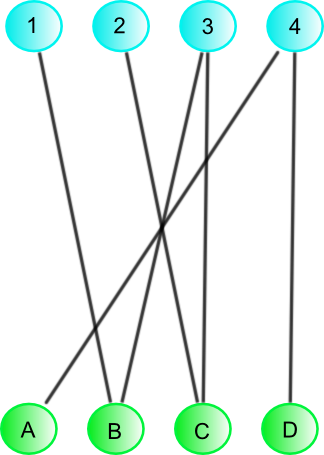
\includegraphics[scale=0.3]{./figuras/BusquedaLocal/reinsercion.png}}     
     \setcounter{subfigure}{1}\hspace{1.0in}
     \subfigure[Buscamos a donde reinsertae al nodo A, delante de D logramos minimizar los cruces]{
     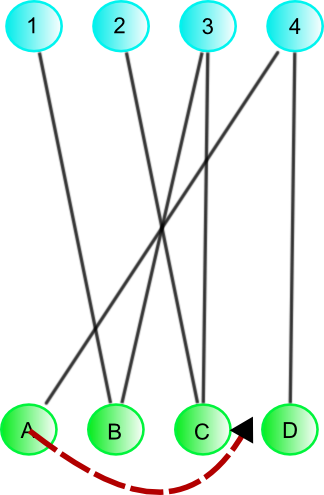
\includegraphics[scale=0.3]{./figuras/BusquedaLocal/reinsercion1.png}}    
     \setcounter{subfigure}{2}
     \subfigure[Movemos al nodo A, no podemos mover a nadie mas de esta partici�n de modo de bajar el n�mero de cruces, por lo cual, pasamos a la siguiente partici�n. Moviendo a 4 no logramos nada, por lo que buscamos mover a 3(1 cruce)]{
     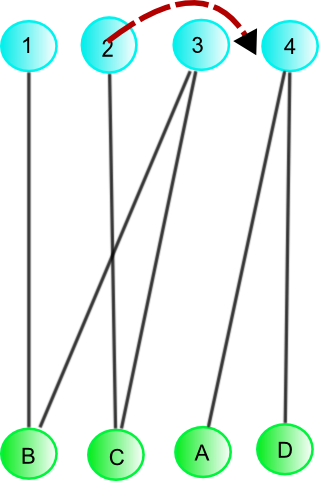
\includegraphics[scale=0.3]{./figuras/BusquedaLocal/reinsercion2.png}}     
     \setcounter{subfigure}{3}\hspace{1.0in}
     \subfigure[Movimos a 3, y ya no queda ninguna mejora por hacer (0 cruces)]{
     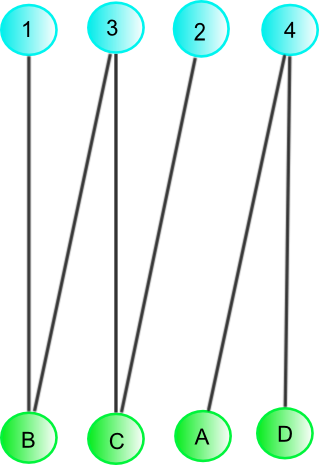
\includegraphics[scale=0.3]{./figuras/BusquedaLocal/reinsercion3.png}}     
\end{figure} 

\subsubsection{Pseudocodigo}
\begin{algorithm}[H]
\caption{Intenta mejorar un dibujo mediante la reinserci�n golosa de nodos}
\begin{algorithmic}[1]
\FOR{cada nodo del dibujo}
\STATE sacar al nodo del mismo
\STATE obtener las posiciones donde es posible insertarlo
\STATE mejoresCruces $\leftarrow$ cruces por ponerlo en la primer posici�n posible
\STATE mejorPosici�n $\leftarrow$ primer posici�n
\FOR{cada posici�n donde se puede poner al nodo}
\STATE crucesActuales $\leftarrow$ cruces por ponerlo en dicha posici�n
\IF{crucesActuales $<$ mejoresCruces}
\STATE mejoresCruces $\leftarrow$ crucesActuales
\STATE mejorPosici�n $\leftarrow$ posici�n actual
\ENDIF
\ENDFOR
\STATE poner al nodo en la mejor posici�n
\ENDFOR
\end{algorithmic}
\end{algorithm} 

\subsection{Busqueda local por intercambio goloso de nodos}
Esta heuristica contempla como soluciones vecinas de un dibujo a aquellas que se pueden obtener por un intercambio v�lido entre dos nodos del dibujo.

\begin{figure}[H]
    \centering
     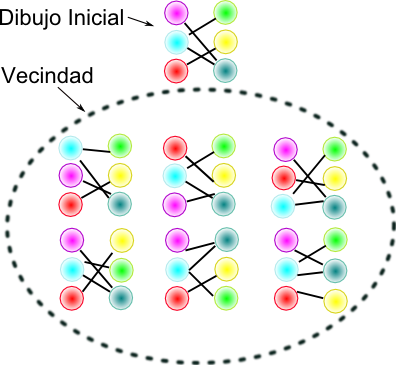
\includegraphics[scale=0.5]{./figuras/BusquedaLocal/vecindad.png}
\end{figure}

Primero se considera la vecindad, consistente en todo posible intercambio de dos nodos (siempre que dicho intercambio no viole el orden relativo de los nodos originales) y luego prueba cual de todos esos intercambios reporta mayor beneficio, es decir reduce mas el n�mero de cruces. Una vez encontrado dicho par, nos movemos a la soluci�n vecina realizando el intercambio de dichos nodos. Al hacerlo terminamos un paso de la busqueda local.

El procedimiento se repite hasta que ning�n intercambio genere una reducci�n en el n�mero de cruces. En cuyo caso decimos que alcanzamos un m�nimo local.

\subsubsection{Pseudocodigo}
\begin{algorithm}[H]
\caption{Intenta mejorar un dibujo mediante intercambio goloso de nodos}
\begin{algorithmic}[1]
\STATE vecindad = \{(x,y) por cada x en alguna particion e y de la misma partici�n, si es v�lido intercambiar x por y\}
\STATE mejorIntercambio $\leftarrow$ ninguno
\STATE crucesPorIntercambio $\leftarrow$ cantidad de cruces del dibujo
\FOR{(x,y) en vecindad}
\STATE crucesVecino $\leftarrow$ cantidad de cruces al intercambiar x e y
\IF{crucesVecino $<$ crucesPorIntercambio}
\STATE mejorIntercambio $\leftarrow$ (x,y)
\STATE crucesPorIntercambio $\leftarrow$ cruces al intercambiar x e y
\ENDIF
\ENDFOR
\IF{mejorIntercambio $\neq$ ninguno}
\STATE realizar el intercambio
\ENDIF
\end{algorithmic}
\end{algorithm} 

\subsection{Busqueda local por inserci�n por mediana}
Una de las heuristicas constructivas que planteamos es la inserci�n de nodos por mediana. Esta heuristica no funcion� bien como esperabamos, ya que si bien era r�pida, generaba mas cruces que las otras heuristicas golosas. Nuestra idea entonces es aplicar el concepto de la mediana, pero como busqueda local.

En este contexto como todos los nodos estan puestos, cada nodo tiene ahora la informaci�n de todos sus adyacentes, es por esta raz�n que creemos que podria funcionar bien el metodo como busqueda local.

Entonces la idea es muy similar a la inserci�n por mediana: tomamos cada nodo de una partici�n y tratamos de moverlo a la posici�n correspondiente a la mediana de las posiciones de sus adyacentes, o la mediana mas o menos uno. Si al moverlo se reducen los cruces lo hacemos. Si esto no ocurre, se lo deja donde esta. A diferencia de la heuristica constructiva, en esta los nodos que estaban en el dibujo inicial tambi�n se intentan ubicar segun sus medianas siempre que esto no rompa el orden relativo que deben guardar.

 Una vez hecho esto para todos los nodos, lo que hacemos es tratar de intercambiar adyacentes, con el objetivo de reducir el n�mero de cruces.

La busqueda termina cuando no es posible reducir el n�mero de cruces ya sea ubicando en la posici�n de la mediana o por intercambio de pares.

\subsubsection{Pseudocodigo}
\begin{algorithm}[H]
\caption{Intenta mejorar un dibujo inserci�n por mediana}
\begin{algorithmic}[1]
\FOR{ cada nodo del dibujo}
\STATE calcular la mediana de las posiciones de los adyacentes al nodo
\STATE mejorPos $\leftarrow$ posicionActual
\STATE mejoreCruces $\leftarrow$ cruces en el dibujo
\FOR{ posicion = mediana -1, mediana, mediana + 1}
\IF{ se puede insertar en esa posici�n  y baja el n�mero de cruces en el dibujo}
\STATE mejorPos $\leftarrow$ posicion
\STATE mejoresCruces $\leftarrow$ cruces en el dibujo al poner al nodo en posicion
\ENDIF
\ENDFOR
\STATE poner al nodo en mejorPos
\ENDFOR
\end{algorithmic}
\end{algorithm} 
